\documentclass[]{article}
\usepackage{lmodern}
\usepackage{amssymb,amsmath}
\usepackage{ifxetex,ifluatex}
\usepackage{fixltx2e} % provides \textsubscript
\ifnum 0\ifxetex 1\fi\ifluatex 1\fi=0 % if pdftex
  \usepackage[T1]{fontenc}
  \usepackage[utf8]{inputenc}
\else % if luatex or xelatex
  \ifxetex
    \usepackage{mathspec}
  \else
    \usepackage{fontspec}
  \fi
  \defaultfontfeatures{Ligatures=TeX,Scale=MatchLowercase}
\fi
\usepackage{color}

% use upquote if available, for straight quotes in verbatim environments
\IfFileExists{upquote.sty}{\usepackage{upquote}}{}
% use microtype if available
\IfFileExists{microtype.sty}{%
\usepackage[]{microtype}
\UseMicrotypeSet[protrusion]{basicmath} % disable protrusion for tt fonts
}{}
\PassOptionsToPackage{hyphens}{url} % url is loaded by hyperref
\usepackage[unicode=true]{hyperref}
\hypersetup{
            pdfborder={0 0 0},
            breaklinks=true}
\urlstyle{same}  % don't use monospace font for urls
\usepackage{graphicx,grffile}
\makeatletter
\def\maxwidth{\ifdim\Gin@nat@width>\linewidth\linewidth\else\Gin@nat@width\fi}
\def\maxheight{\ifdim\Gin@nat@height>\textheight\textheight\else\Gin@nat@height\fi}
\makeatother
% Scale images if necessary, so that they will not overflow the page
% margins by default, and it is still possible to overwrite the defaults
% using explicit options in \includegraphics[width, height, ...]{}
\setkeys{Gin}{width=\maxwidth,height=\maxheight,keepaspectratio}
\IfFileExists{parskip.sty}{%
\usepackage{parskip}
}{% else
\setlength{\parindent}{0pt}
\setlength{\parskip}{6pt plus 2pt minus 1pt}
}
\setlength{\emergencystretch}{3em}  % prevent overfull lines
\providecommand{\tightlist}{%
  \setlength{\itemsep}{0pt}\setlength{\parskip}{0pt}}
\setcounter{secnumdepth}{0}
% Redefines (sub)paragraphs to behave more like sections
\ifx\paragraph\undefined\else
\let\oldparagraph\paragraph
\renewcommand{\paragraph}[1]{\oldparagraph{#1}\mbox{}}
\fi
\ifx\subparagraph\undefined\else
\let\oldsubparagraph\subparagraph
\renewcommand{\subparagraph}[1]{\oldsubparagraph{#1}\mbox{}}
\fi

% set default figure placement to htbp
\makeatletter
\def\fps@figure{htbp}
\makeatother


\date{}

\begin{document}

\subsubsection{Statistical Mechanics}\label{statistical-mechanics}

A lot can be accomplished without ever acknowledging the existence of
molecules. Indeed, much of thermodynamics exists for just this purpose.
Thermodynamics permits us to explain and predict phenomena that depend
crucially on the fact that our world comprises countless molecules, and
it does this without ever recognizing their existence. In fact,
establishment of the core ideas of thermodynamics predates the general
acceptance of the atomic theory of matter. Thermodynamics is a formalism
with which we can organize and analyze macroscopic experimental
observations, so that we have an intelligent basis for making
predictions from limited data. Thermodynamics was developed to solve
practical problems, and it is a marvelous feat of science and
engineering.

Of course, to fully understand and manipulate the world we must deal
with the molecules. But this does not require us to discard
thermodynamics. On the contrary, thermodynamics provides the right
framework for constructing a molecular understanding of macroscopic
behavior. Thermodynamics identifies the interesting macroscopic features
of a system. \emph{Statistical mechanics} is the formalism that connects
thermodynamics to the microscopic world. Remember that a statistic is a
quantitative measure of some collection of objects. An observation of
the macroscopic world is necessarily an observation of some statistic of
the molecular behaviors. The laws of thermodynamics derive largely from
laws of statistics, in particular the simplifications found in the
statistics of large numbers of objects. These objects---molecules---obey
mechanical laws that govern their behaviors; these laws, through the
filter of statistics, manifest themselves as macroscopic observables
such as the equation of state, heat capacity, vapor pressure, and so on.
The correct mechanics of molecules is of course quantum mechanics, but
in a large number of situations a classical treatment is completely
satisfactory.

A principal aim of molecular simulation is to permit calculation of the
macroscopic behaviors of a system that is defined in terms of a
microscopic model, a model for the mechanical interactions between the
molecules. Clearly then, statistical mechanics provides the appropriate
theoretical framework for conducting molecular simulations. In this
section we summarize from statistical mechanics the principal ideas and
results that are needed to design, conduct, and interpret molecular
simulations. Our aim is not to be rigorous or comprehensive in our
presentation. The reader needing a more detailed justification for the
results given here is referred to one of the many excellent texts on the
topic. Our focus at present is with thermodynamic behaviors of
equilibrium systems, so we will not at this point go into the ideas
needed to understand the microscopic origins of transport properties,
such as viscosity, thermal conductivity and diffusivity.

\subsubsection{Ensembles}\label{ensembles}

A key concept in statistical mechanics is the \emph{ensemble}. An
ensemble is a collection of microstates of system of molecules, all
having in common one or more extensive properties. Additionally, an
ensemble defines a probability distribution $\pi$ accords a weight to each
element (microstate) of the ensemble. These statements require some
elaboration. A \emph{microstate} of a system of molecules is a complete
specification of all positions and momenta of all molecules
(\emph{i.e.}, all atoms in all molecules, but for brevity we will leave
this implied). This is to be distinguished from a thermodynamic state,
which entails specification of very few features, \emph{e.g.} just the
temperature, density and total mass. An extensive quantity is used here
in the same sense it is known in thermodynamics---it is a property that
relates to the total amount of material in the system. Most frequently
we encounter the total energy, the total volume, and/or the total number
of molecules (of one or more species, if a mixture) as extensive
properties. Thus an ensemble could be a collection of all the ways that
a set of $N$ molecules could be arranged (specifying the location
and momentum of each) in a system of fixed volume. As an example, in
Fig.~\ref{fig:NVT} we show a few elements of an ensemble of five molecules.
\begin{figure}

\includegraphics[width=\textwidth]{StatMech_figures/image001}
\caption{\label{fig:NVT}A few members of the $NVT$ ensemble, for $N = 5$.}
\end{figure}

If a particular extensive variable is not selected as one that all
elements of the ensemble have in common, then all physically possible
values of that variable are represented in the collection. For example,
Fig.~\ref{fig:NPT} presents some of the elements of an ensemble in which
only the total number of molecules is fixed. The elements are not
constrained to have the same volume, so all possible volumes from zero
to infinity are represented. Likewise in both Figs. \ref{fig:NVT} and \ref{fig:NPT} the
energy is not selected as one of the extensive variables held fixed. So we
see among the displayed elements configurations in which molecules
overlap. These high-energy states are included in the ensemble, even
though we do not expect them to arise in the real system. The likelihood
of observing a given element of an ensemble---its physical
relevance---comes into play with the probability distribution $\pi$ that
forms part of the definition of the ensemble.
\begin{figure}
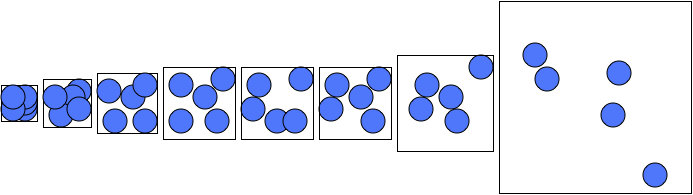
\includegraphics[width=\textwidth]{Statmech_figures/image111}
\caption{\label{fig:NPT}A few members of the \emph{NPT} ensemble, for $N = 5$.}
\end{figure}


Any extensive property omitted from the specification of the ensemble is
replaced by its conjugate intensive property. So, for example, if the
energy is not specified to be common to all ensemble elements, then
there is a temperature variable associated with the ensemble. These
intensive properties enter into the weighting distribution $\pi$ in a way
that will be discussed shortly. It is common to refer to an ensemble by
the set of independent variables that make up its definition. Thus the
$TVN$ ensemble collects all microstates of the same volume and molecular
number, and has temperature as the third independent variable. The more
important ensembles have specific names given to them. These are:

\begin{itemize}
\item
  Microcanonical ensemble (\emph{EVN})
\item
  Canonical ensemble (\emph{TVN})
\item
  Isothermal-isobaric ensemble (\emph{TPN})
\item
  Grand-canonical ensemble (\emph{TV$\mu$})
\end{itemize}
%Seems like this should cross-reference the SimElements document which has a table on these.

These are summarized in Fig.~\ref{fig:ensembles}, with a schematic of the elements
presented for each ensemble.

\begin{figure}
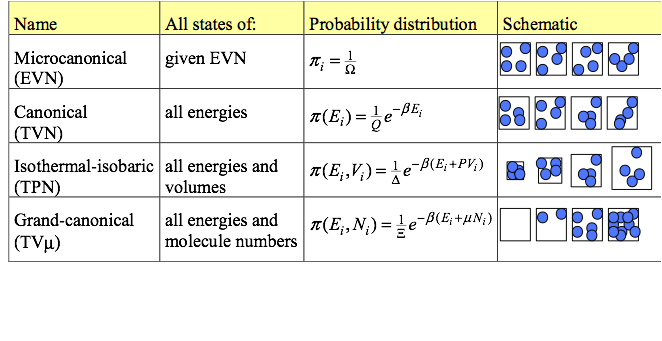
\includegraphics[width=\textwidth]{StatMech_figures/image003}
\caption{\label{fig:ensembles}Commonly used ensembles.}
\end{figure}
%Not all symbols used in figure are defined in this chapter, which seems less than ideal; probably need to be in caption.


\subsubsection{Postulates}\label{postulates}

Statistical mechanics rests on two postulates:

\begin{enumerate}
\def\labelenumi{\arabic{enumi}.}
\item
  \emph{Postulate of equal \emph{a priori} probabilities}. This
  postulate applies to the microcanonical (\emph{EVN}) ensemble. Simply put, it
  asserts that the weighting function $\pi$ is a constant in the
  microcanonical ensemble. All microstates of equal energy are accorded
  the same weight.
\item
  \emph{Postulate of ergodicity}. This postulate states that the
  time-averaged properties of a thermodynamic system---the properties
  manifested by the collection of molecules as they proceed through
  their natural dynamics---are equal to the properties obtained by
  weighted averaging over all microstates in the ensemble.
\end{enumerate}

The postulates are arguably the least arbitrary statements that one
might make to begin the development of statistical mechanics. They are
non-trivial but almost self-evident, and it is important that they be
stated explicitly. They pertain to the behavior of an isolated system,
so they eliminate all the complications introduced by interactions with
the surroundings of the system. The first postulate says that in an
isolated system there are no special microstates; each microstate is no
more or less important than any other.

Note that conservation of energy requires that the dynamical evolution
of a system proceeds through the elements of the microcanonical
ensemble. Measurements of equilibrium thermodynamic properties can be
taken during this process, and these measurements relate to some
statistic (\emph{e.g.}, an average) for the collective system (later in
this section we consider what types of ensemble statistics correspond to
various thermodynamic observables). Of course, as long as we are not
talking about dynamical properties, these measurements (statistics) do
not depend on the order in which the elements of the ensemble are
sampled. This point cannot be disputed. What is in question, however, is
whether the dynamical behavior of the system will truly sample all (or a
fully representative subset of all) elements of the microcanonical
ensemble. In fact, this is not the outcome in many experimental
situations. The collective dynamics may be too sluggish to visit all
members of the ensemble within a reasonable time. In these cases we
fault the dynamics. Instead of changing our definition of equilibrium to
match each particular experimental situation, we maintain that
equilibrium behavior is by definition that which samples a fully
representative set of the elements of the governing ensemble. From this
perspective the ergodic postulate becomes more of a definition than an
axiom.

\subsubsection{Other ensembles}\label{other-ensembles}

A statistical mechanics of isolated systems is not convenient. We need
to treat systems in equilibrium with thermal, mechanical, and chemical
reservoirs. Much of the formalism of statistical mechanics is devised to
permit easy application of the postulates to non-isolated systems. This
parallels the development of the formalism of thermodynamics, which
begins by defining the entropy as a quantity that is maximized for an
isolated system at equilibrium. Thermodynamics then goes on to define
the other thermodynamic potentials, such as the Helmholtz and Gibbs free
energies, which are found to obey similar extremum principles for
systems at constant temperature and/or pressure.

The ensemble concept is central to the corresponding statistical
mechanics development. For example, a closed system at fixed volume, but
in thermal contact with a heat reservoir, samples a collection of
microstates that make up the canonical ensemble. The approach to
treating these systems is again based on the ensemble average. The
thermodynamic properties of an isothermal system can be computed as
appropriate statistics applied to the elements of the canonical
ensemble, without regard to the microscopic dynamics. Importantly, the
weighting applied to this ensemble is not as simple as that postulated
for the microcanonical ensemble; but through an appropriate construction
it can be derived from the principle of equal \emph{a priori}
probabilities. We will not present this derivation here, except to
mention that the only additional assumption it invokes involves the
statistics of large samples. Details may be found in standard texts in
statistical mechanics.

The weighting distributions for the four major ensembles are included in
the table of Fig.~\ref{fig:ensembles}. Let us examine the canonical-ensemble form:

\[\pi \left( {{E_i};T,V,N} \right) = \frac{1}{{Q(T,V,N)}}{e^{ - \beta {E_i}}}.\]

The symbol $\beta$ here (and universally in the statistical mechanics
literature) represents $1/k_{\rm B}T$, where $k_{\rm B}$ is Boltzmann's constant; in this
manner the temperature influences the properties of the ensemble. The
term is known as the \emph{Boltzmann factor} of the energy
\emph{E}\textsubscript{i}. Note that the weighting accorded to a
microstate depends only on its energy; states of equal energy have the
same weight. The normalization constant \emph{Q} is very important, and
will be discussed in more detail below. Note also that the quantity $E/T$,
which appears in the exponent, in thermodynamics is the term subtracted
from the entropy to form the constant-temperature Legendre transform,
commonly known as the Helmholtz free energy (divided by $T$). This
weighting distribution makes sense physically. Given that we must admit
all microstates, regardless of their energy, we now see that the
unphysical microstates are excluded not by fiat but by their weighting.
Microstates with overlapping molecules are of extremely high energy. The
Boltzmann factor is practically zero in such instances, and thus the
weighting is negligible. As the temperature increases, higher-energy
microstates have a proportionately larger influence on the ensemble
averages.

Turning now to the \emph{NPT}-ensemble weighting function, we begin to uncover
a pattern:
\[\pi ({E_i},{V_i};T,P,N) = \frac{1}{{\Delta (T,P,N)}}{e^{ - \beta {E_i} - \beta P{V_i}}}\]

The weight depends on the energy and the volume of the microstate
(remember that this isothermal-isobaric ensemble includes microstates of
all possible volumes). The pressure influences the properties through
its effect on the weighting distribution. The term in the exponent is
again that which is subtracted from the entropy to define the \emph{NPT}
Legendre transform, the Gibbs free energy. We now turn to the connection
between the thermodynamic potential and the normalization constant of
the distribution.

\subsubsection{Partition functions and bridge
equations}\label{partition-functions-and-bridge-equations}

The connection to thermodynamics is yet to be made, and without it we
cannot relate our ensemble averages to thermodynamic observables. As
alluded above, the connection comes between the thermodynamic potential
and the normalization constants of the weighting functions. These
factors have a fancy name: we know them as \emph{partition functions},
but the German name is more descriptive: \emph{Zustandssumme}, which means
``sum over states''. Because they normalize the weighting function, they
represent a sum over all microstates of the ensemble, summing the
Boltzmann factor for each element. The bridge equations relating these
functions to their thermodynamic potentials are summarized in
Fig.~\ref{fig:bridgeEqns}. We assert the results, again without proof. In what follows, we
show several examples of their plausibility, in that they give very
sensible prescriptions for the ensemble averages needed to evaluate some
specific thermodynamic properties from molecular behaviors.

\begin{figure}
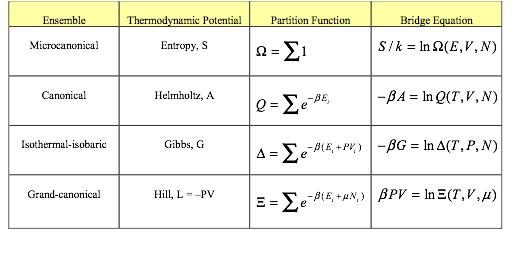
\includegraphics[width=\textwidth]{StatMech_figures/image011}
\caption{\label{fig:bridgeEqns}Relation between commonly used ensemble and thermodynamic free energies.}
\end{figure}

\subsubsection{Ensemble averaging}\label{ensemble-averaging}

Let us begin now to become more specific in what we mean by ensemble
averaging. The usual development begins with quantum mechanics, because
in quantum mechanics the elements of an ensemble form a discrete set, as
given by the solutions of the time-independent Schr{\"o}dinger equation.
They may be infinite in number, but they are at least countably
infinite, and therefore it is possible to imagine gathering a set of
these discrete states to form an ensemble. The transition to classical
mechanics then requires an awkward (or a least tedious) handling of the
conversion to a continuum. We will bypass this process and move straight
to classical mechanics, appealing more to concepts rather than rigor in
the development.

For a given $N$ and $V$, an element of an ensemble corresponds to a point in
classical \emph{phase space}, $\Gamma$. Phase space refers to the (highly
dimensional) space of all positions and momenta of (all atoms of) all
molecules: $\Gamma  = ({{\bf{r}}^N},{{\bf{p}}^N})$. Each molecule occupies a space of dimension \emph{d},
meaning that each \textbf{r} and \textbf{p} is a \emph{d}-dimensional
vector, and $\Gamma$ is then a 2\emph{dN}-dimensional space (\emph{e.g.}, for
100 atoms occupying a three-dimensional space, $\Gamma$ forms a 600-dimensional
space). We consider now an observable A($\Gamma$) defined for each point in
phase space, for example the total intermolecular energy. For a discrete
set of microstates, the ensemble average of $A$ is
\[\left\langle A \right\rangle  = \sum {{A_i}{\pi _i}} \]
In the continuum phase space, for the canonical ensemble this average
takes the form
\[\left\langle A \right\rangle  = \frac{1}{Q} \frac{1}{h^{dN}N!}\int {d{{\bf p}^N}\int {d{{\bf r}^N}A({{\bf p}^N},{{\bf r}^N})} {e^{ - \beta E({{\bf p}^N},{{\bf r}^N})}}} \]
The sum becomes an integral over all positions and momenta. Every
possible way of arranging the atoms in the volume $V$ is included;
likewise all possible momenta, from minus- to plus-infinity are
included. The Boltzmann weighting factor filters out the irrelevant
configurations. Two other terms arise in the integral. The factor
involving Planck's constant \emph{h} is an inescapable remnant of the
quantum mechanical origins of the ensemble. As a crude explanation, one
might think of the transition to the classical continuum as a smearing
out of each of the true quantum states of the system. The ``distance''
between each adjacent point in quantum phase space is proportional to
$h$, so the volume of these smeared-out regions goes as
$h^{3N}$, and this must be divided out to
renormalize the sum. Note also that the term in $h$ cancels the
dimensions of the integration variables
${\bf r}^N{\bf p}^N$. The other term in the
integral, $N!$, eliminates overcounting of the microstates. Each
bona fide, unique element of the ensemble arises in this phase-space
integral \emph{N}! times. This happens because all molecules move over
all of the system volume, and multiple configurations arise that differ
only in the labeling of the molecules. For indistinguishable molecules
the labels are physically irrelevant, so these labeling permutations
should not all contribute to the phase-space integral. The expression
for the canonical-ensemble partition function follows likewise
\[Q = \frac{1}{h^{dN}N!}\int {d{{\bf p}^N}\int {d{{\bf r}^N}} {e^{ - \beta E({{\bf p}^N},{{\bf r}^N})}}} \]
With a suitable choice of coordinates, it is possible to separate the
total energy $E$ into a kinetic part $K$ that depends only on
the momentum coordinates, and a potential part $U$ that likewise
depends only on the position coordinates:
\[E({{\bf{p}}^N},{{\bf{r}}^N}) = K({{\bf{p}}^N}) + U({{\bf{r}}^N}).\]
The kinetic energy is quadratic in the momenta:
\[K({{\bf p}^N}) = \sum\nolimits_i {|{\bf p}_i|^2/2{m_i}}, \]
and this contribution can be treated analytically in the partition
function:
\begin{align}
Q &= \frac{1}{{h^{dN}}}\frac{1}{N!}\int {d{{\bf p}^N}{e^{ - \beta \sum {|{\bf p}_i|^2/2m} }}\int {d{{\bf r}^N}} {e^{ - \beta U({{\bf r}^N})}}} \nonumber\\
 &= \frac{1}{{\Lambda ^{dN}}}\frac{1}{N!}\int {d{{\bf r}^N}} {e^{ - \beta U({{\bf r}^N})}}\nonumber\\
 &= \frac{1}{{\Lambda ^{dN}}}\frac{1}{N!}{Z_N}\nonumber
\end{align}
where $\Lambda \equiv h/\sqrt{2\pi mk_{\rm B}T}$ is known as the thermal de Broglie wavelength, and
$Z_N$ as defined here is the \emph{configurational
integral} (some authors define it to not include the ${N}!$ term).
The momentum contributions drop out of ensemble averages of observables
that depend only on coordinates:
\[\left\langle A \right\rangle  = \frac{1}{{{Z_N}}}\frac{1}{{N!}}\int {d{{\bf{r}}^N}A({{\bf{r}}^N}){e^{ - \beta U({{\bf{r}}^N})}}} \]
This formula sees broad use in molecular simulation.

\subsubsection{Time Averaging and Ergodicity (A brief
aside)}\label{time-averaging-and-ergodicity-a-brief-aside}

The ergodic postulate relates the ensemble average to a time average, so
it is worthwhile to cast the time average in an explicit mathematical
form. This type of average becomes important when considering the
molecular-dynamical behavior that underlies macroscopic transport
processes. A full treatment of the topic is given elsewhere in these notes.

The time average is taken over all states encountered in a dynamical
trajectory of the system. It can be written thus:
\[\bar A = \mathop {\lim }\limits_{t \to \infty } \frac{1}{t}\int\limits_0^t {A\left( {{{\bf{p}}^N}(t),{{\bf{r}}^N}(t);{{\bf{p}}^N}(0),{{\bf{r}}^N}(0)} \right)} dt'.\]
The positions and momenta are given as functions of time $\left( {{{\bf{r}}^N}(t),{{\bf{p}}^N}(t)} \right)$ via the
governing mechanics. As indicated, these depend on their values at the
initial time, \emph{t} = 0. However, if the dynamics is ergodic (it can
reach all elements of the corresponding microcanonical ensemble), then
in the limit of infinite time the initial conditions become irrelevant
(with the notable qualification that the initial conditions specify the
total energy, and thus designate the particular microcanonical (\emph{EVN})
ensemble that is sampled; a more precise statement is that the time
average is independent of which member of a given microcanonical
ensemble is chosen as the initial condition).

As stated above, if a dynamical process is capable of reaching a
representative set elements of an ensemble (since the number of elements
is infinite, the complete set of states can never be reached), we say
that the process is \emph{ergodic}. Figure~\ref{fig:ergodicity} shows a schematic
representation of a case in which the dynamics is not ergodic. It is
useful to generalize this idea to processes that are not necessarily
following the true dynamics of the system. Any algorithm that purports
to generate a representative set of configurations from the ensemble may
be viewed in terms of its ergodicity. It is ergodic if it does generate a
representative sample (in the time it is given to proceed).

\begin{figure}
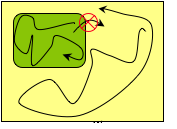
\includegraphics[width=\textwidth]{StatMech_figures/image036}
\caption{\label{fig:ergodicity}Illustration of ergodicity. Plane represents phase space, and two trajectories are shown. If non-ergodic, there are regions of phase space that are not accessible by both trajectories, as suggested by the green subregion.}
\end{figure}

%An applet demonstrating non-ergodic behavior is presented in Illustration 6.

\subsubsection{Simple Thermodynamic
Averages}\label{simple-thermodynamic-averages}

\paragraph{Internal energy}\label{internal-energy}

The ensemble average of the internal energy must certainly correspond to
the thermodynamic quantity known as the internal energy. How could there
be any disputing this? Well, let us not take it for granted, and instead
set about proving this result from the preceding developments. It is
actually very simple to do, and it sets the stage for more difficult
derivations of the same type.

The Gibbs-Helmholtz equation of thermodynamics states:
\[{E_{{\rm{internal}}}} = {\left( {\frac{{\partial (A/{k_{\rm B}}T)}}{{\partial (1/{k_{\rm B}}T)}}} \right)_{V,N}}\]
If we apply the canonical-ensemble bridge equation to write the
Helmholtz free energy \emph{A} in terms of the partition function we
have the following
\begin{align*}
{E_{{\rm{internal}}}} &= {\left( {\frac{{\partial (A/k_{\rm B}T)}}{{\partial (1/k_{\rm B}T)}}} \right)_{V,N}}\\
 &=  - \frac{{\partial \ln Q}}{{\partial \beta }}\\
 &=  - \frac{1}{Q}\frac{\partial }{{\partial \beta }}\left[\frac{1}{h^{dN}N!}\int {d{{\bf p}^N}\int {d{{\bf r}^N}} {e^{ - \beta E({{\bf p}^N},{{\bf r}^N})}}} \right]\\
 &=  + \frac{1}{Q}{\frac{1}{h^{dN}N!}\int {d{{\bf p}^N}\int {d{{\bf r}^N}E({{\bf p}^N},{{\bf r}^N})} {e^{ - \beta E({{\bf p}^N},{{\bf r}^N})}}}} \\
 &= \left\langle E \right\rangle 
\end{align*}
which is what we set out to prove. Other simple averages, such as the
average volume in the \emph{NPT} ensemble, or the average number of molecules
in the grand-canonical ensemble, can be confirmed to connect to the
expected thermodynamic observables in a similar fashion. We leave this
verification as an exercise to the reader.

We can take our result for the energy one step further by introducing
the separation of the energy into its kinetic and potential
contributions, as discussed above:
\begin{align*}
\left\langle E \right\rangle  &= \frac{1}{Q}\frac{1}{{{h^{dN}}N!}}\int {d{{\bf{p}}^N}\int {d{{\bf{r}}^N}\left[ {K({{\bf{p}}^N}) + U({{\bf{r}}^N})} \right]} {e^{ - \beta E({{\bf{p}}^N},{{\bf{r}}^N})}}} \\
 &= \frac{1}{{{\Lambda ^{dN}}}}\int {d{{\bf{p}}^N}\left( {\sum {{\textstyle{{{{\left| {{{\bf{p}}_i}} \right|}^2}} \over {2{m_i}}}}} } \right){e^{ - \beta \sum {{{\left| {{{\bf{p}}_i}} \right|}^2}/2{m_i}} }}}  + \frac{1}{{{Z_N}N!}}\int {d{{\bf{r}}^N}U({{\bf{r}}^N}){e^{ - \beta U({{\bf{r}}^N})}}} \\
 &= \frac{d}{2}Nk_{\rm B}T + \left\langle U \right\rangle 
\end{align*}
So the kinetic-energy contribution can be treated analytically, and we
arrive at the well-known result that each configuration coordinate
contributes $k_{\rm B}T/2$ to the internal kinetic energy. This result is known as
the principle of equipartition, indicating that the kinetic energy
distributes equally among all microscopic degrees of freedom.

If the potential energy is zero, the system behaves as an ideal gas and
the total internal energy is just that given by the kinetic
contribution. In many circumstances the simplicity of the kinetic part
leads us to ignore it while we focus on the more interesting potential
contribution. It then becomes easy to forget the kinetic part
altogether, and to speak of the potential energy as if it were the only
contributor to the internal energy. The tacit understanding is that we
all know the kinetic part is there and should be added in if the
internal energy is needed for any practical application (\emph{e.g.},
computing a heating requirement).

\paragraph{Temperature}\label{temperature}

Many simulations are conducted in constant-temperature ensembles, and
there is no need to measure the temperature. However, elementary
molecular dynamics simulations sample the microcanonical ensemble, and
thus the temperature is not a quantity known \emph{a priori}. In this
ensemble the total energy is constant, but this energy continually
redistributes between kinetic and potential forms. The standard means
for measuring the temperature rests on the notion of equipartition,
discussed in the previous section. Temperature is expressed in terms of
an average of the kinetic energy, thus:
\[\left\langle T \right\rangle  = \frac{1}{dNk_{\rm B}}\left\langle {\sum\limits_{i = 1}^N \frac{\left| \bf{p}_i \right|^2} {m_i}} \right\rangle \]

Evans has developed an expression for the appropriate ensemble
average needed to evaluate the temperature. His approach does not rely
on equipartition, but instead appeals to the more fundamental definition
of temperature as the change in the entropy with energy in an isolated
system. We will present this formulation later.

\paragraph{Pressure}\label{pressure}

Derivation of a working equation for the pressure is much trickier.
In one approach, the pressure may be computed as an average of the momentum
flux arising from the collisions of atoms with the walls
containing them. However, we use periodic boundary
conditions to conduct simulations without walls, and this leaves us with
a need for another route to measurement of the pressure in our
simulations. We follow the same approach we introduced to connect the
thermodynamic internal energy to an ensemble average, beginning now with
the thermodynamic expression for the pressure:
\begin{align*}
P &=  - {\left( {\frac{{\partial (A/kT)}}{{\partial V}}} \right)_{T,N}}\\
 &= \frac{{\partial \ln Q}}{{\partial V}}\\
 &= \frac{1}{Q}\frac{\partial }{{\partial V}}\left[ {\frac{1}{{{h^{3N}}N!}}\int {d{{\bf{p}}^N}\int {d{{\bf{r}}^N}} {e^{ - \beta E({{\bf{p}}^N},{{\bf{r}}^N})}}} } \right]
\end{align*}
Where is $V$ in the phase-space integral? It lies in the limits of
integration of the position integrals. There is a standard trick used to
move the volume dependence into a position where it is more easily
differentiated. It is worth describing this idea here, as it arises
again in the simulation of systems at constant pressure, in which the
volume fluctuates. Before going further, let us point out that the
volume does not enter into the momentum integrals or the kinetic
contribution to the energy. Upon separating these parts in the manner
shown above the volume derivative causes them to drop out, so we can
simplify our starting point a bit by removing them now, thus:
\[P = \frac{1}{{{Z_N}}}\frac{\partial }{{\partial V}}\left[ {\int_{{V^N}} {d{{\bf{r}}^N}{e^{ - \beta U({{\bf{r}}^N})}}} } \right]\]
We now scale all the position coordinates by the linear dimension
$L$ of the volume ($V = L^d$). To fix ideas,
imagine that the volume is cubic in shape, as shown in Fig.~\ref{fig:Vscaling}.
Taking for example a 2-dimensional space, we define scaled coordinates ${\bf{s}} = ({s_x},{s_y}) = ({r_x}/L,{r_y}/L) = {\bf{r}}/V$
(we introduce some useful shorthand notation here) and rewrite the
configuration integral over a unit volume
\[P = \frac{1}{{{Z_N}}}\frac{\partial }{{\partial V}}\left[ {\int_1 {d{{(V{\bf{s}})}^N}{e^{ - \beta U({{(V{\bf{s}})}^N})}}} } \right]\]
The internal energy \emph{U} depends on volume through the pair
separation vectors $\bf{r} = (V\bf{s})$. Remember that the force
on a molecule is the gradient of the potential
\[{\bf{F}} =  - \left( {\frac{{\partial U}}{{\partial {r_x}}}{{{\bf{\hat e}}}_x} + \frac{{\partial U}}{{\partial {r_y}}}{{{\bf{\hat e}}}_y}} \right)\]

\begin{figure}
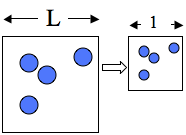
\includegraphics[width=\textwidth]{StatMech_figures/image049}
\caption{\label{fig:Vscaling}Scaling the volume to a unit size.}
\end{figure}

and note that our coordinate scaling now maps changes in the volume to
changes in the spatial positions of all the molecules, and through this
process effects a change in the energy. Consequently, the volume
derivative can be expressed in terms of the forces on the molecules:
\begin{align*}
\frac{\partial }{{\partial V}}U(V{{\bf{s}}_1},...,V{{\bf{s}}_N}) &= \sum\limits_{i = 1}^N {\left( {\frac{{\partial U}}{{\partial \left( {L{s_{i,x}}} \right)}}\frac{{d\left( {L{s_{i,x}}} \right)}}{{dV}} + \frac{{\partial U}}{{\partial \left( {L{s_{i,y}}} \right)}}\frac{{d\left( {L{s_{i,y}}} \right)}}{{dV}}} \right)} \\
 &= \frac{1}{{Vd}}\sum\limits_{i = 1}^N {\left( {\frac{{\partial U}}{{\partial {r_{i,x}}}}{r_{i,x}} + \frac{{\partial U}}{{\partial {r_{i,y}}}}{r_{i,y}}} \right)} \\
 &= \frac{1}{{Vd}}\sum\limits_{i = 1}^N {{{\bf{F}}_i} \cdot {{\bf{r}}_i}} 
\end{align*}
If we define the \emph{virial} $W$:
\[W \equiv \frac{1}{d}\sum\limits_{i = 1}^N {{{\bf{F}}_i} \cdot {{\bf{r}}_i}} \]
then on executing all the volume derivatives needed for the pressure, we
obtain
\[P = \frac{{NkT}}{V} + \frac{1}{V}\left\langle W \right\rangle. \]
The first part is just the ideal-gas contribution, while the second term
entails the ensemble average. This is known as the virial formula for
the pressure (not to be confused with the low-density expansion of the
pressure, known as the virial equation of state).

One more step is needed to render this result into a useful form. If the
interactions between the molecules are pairwise additive---meaning that
the potential energy can be written as a sum of terms each involving the
coordinate of no more than two molecules---then the force on a molecule
can likewise be decomposed into a sum of pair terms. Considering that
forces between molecules are equal in magnitude and opposite in
direction, the virial can be expressed as a pair sum too:
\[W = \frac{1}{d}\sum\limits_{i = 1}^N {\sum\limits_{j < i} {{{\bf{r}}_{ij}} \cdot {{\bf{F}}_{ij}}} } \]
where ${{\bf{r}}_{ij}} \equiv {{\bf{r}}_i} - {{\bf{r}}_j}$ and ${\bf F}_{ij}$ is the force that molecule
\emph{j} exerts on molecule \emph{i}. For spherically symmetric
intermolecular potentials, $u({{\bf{r}}_{ij}}) = u(|{{\bf{r}}_{ij}}|) = u(r)$, and this simplifies further
\begin{align*}
W &=  - \frac{1}{d}\sum\limits_{i = 1}^N {\sum\limits_{j < i} {{r_{ij}}\frac{{du({r_{ij}})}}{{d{r_{ij}}}}} } \\
 &=  - \frac{1}{d}\sum\limits_{i = 1}^N {\sum\limits_{j < i} {w(r)} } 
\end{align*}
Measurements of the pressure by molecular simulation are usually not
accomplished to the same precision as measurements of the energy.
Adjacent molecules tend to position themselves about each other at the
point where their mutual force is zero, which coincides with the minimum
of their pair energy. This means that that there are a substantial
number of pair energies that have their maximum possible magnitude. In
contrast, many contributions to the pressure are from pairs having
nearly zero force, or with positive and negative contributions that tend
to cancel.

These results for the pressure are valid equally to hard and soft
potentials, but their application to hard potentials requires a bit of
additional thinking. For hard
potentials the force is zero except at the moment of impact, where it is
infinite for an instant in time. The time integral of the force over
this instant is the finite impulse that the spheres apply to each other,
and it is this impulse that must be averaged to get the pressure.
Referring to the material presented earlier on hard-sphere collisions,
we have
\begin{align*}
\int\limits_{\rm{collision}} {{{\bf{r}}_{12}} \cdot {{\bf{f}}_{12}}dt}  &= {{\bf{r}}_{12}} \cdot \Delta {\bf{p}}\\
 &= {m_R}{{\bf{v}}_{12}} \cdot {{\bf{r}}_{12}}
\end{align*}
Contributions to the average needed for the pressure are made only at
each collision, so the pressure can be computed by summing this quantity
over all collisions
\[\left\langle W \right\rangle  =  - \frac{1}{{td}}\sum\limits_{\rm collisions} {{m_{R,ij}}{{\bf{v}}_{ij}} \cdot {{\bf{r}}_{ij}}} \]
Note the velocities used here are those before the collision, when ${\bf{v}} \cdot {\bf{r}} < 0$;
also, $t$ in this equation is the total simulation time elapsed
during all the collisions in the sum.

\paragraph{Entropy and free energy}\label{entropy-and-free-energy}

At first glance it seems that the free energy is the simplest of all
properties to evaluate by molecular simulation. After all, the bridge
equation, the fundamental equation connecting thermodynamics to the
partition function, gives the free energy explicitly. The problem is not
one of principle, but of practice. For (almost) all interesting systems,
the phase-space integral that defines the partition function cannot be
evaluated directly by any means. It is certainly too complex to handle
analytically, and it is even too difficult to treat numerically. 
%The applet in Illustration 8 should convey a real sense of the problem. 
Any
methodical algorithm (\emph{e.g.}, Simpson's rule) applied to this
high-dimensional integral will take eons to complete. The problem is
discussed further in the section on Monte Carlo simulation.

One might object that the same problem accompanies the evaluation of any
ensemble average. It is computationally impossible to perform a complete
sum over all elements of the ensemble, so how can any average be
computed? The difference is that ensemble averages do not require all
members to be counted in the average; it requires only that a
representative sample be examined. The ensemble average is a sum of
individual observations of a property defined for each element of the
ensemble. In contrast, the free energy is a property of the \emph{entire
ensemble}. The entropy, for example, is the total number of elements in
the ensemble. A representative sample of the ensemble cannot be used to
tell how many members are left outside the sample. To evaluate the free
energy one must, in principle, enumerate all of the elements of the
corresponding ensemble.

The trick to calculating free energies by molecular simulation is to
settle for computing \emph{free-energy differences}. This is not nearly
as hard as computing an absolute free energy. Still there are many
pitfalls, and free-energy calculation is a highly specialized technique
in molecular simulation. We reserve its discussion for another part of
these notes.

\paragraph{Second-derivative
properties}\label{second-derivative-properties}

The heat capacity is an example of a
``2\textsuperscript{nd}-derivative'' property, in that it can be
expressed as a second-derivative of a thermodynamic potential
\[{C_v} = {\left( {\frac{{\partial E}}{{\partial T}}} \right)_{V,N}} =  - k{\beta ^2}{\left( {\frac{{{\partial ^2}(\beta A)}}{{\partial {\beta ^2}}}} \right)_{V,N}}\]
The formula for evaluating it by molecular simulation follows in simple
way from the expression for the average energy. For convenience in what
follows we express the $T$-derivative as a derivative of $\beta = 1/k_{\rm B}T$:
\begin{align*}
{C_v} &=  - k_{\rm B}{\beta ^2}{\left( {\frac{{\partial \left\langle E \right\rangle }}{{\partial \beta }}} \right)_{V,N}}\\
 &=  - k_{\rm B}{\beta ^2}\frac{\partial }{{\partial \beta }}\frac{1}{{Q({\color{red} \beta} )}}\int {d{{\bf r}^N}d{{\bf p}^N}} E{e^{ - {\color{red} \beta} E}}.
\end{align*}

The dependence on $\beta$ is highlighted in red. There are two parts, one
involving the integrand, and the other involving the normalizing
partition function. Straightforward manipulations lead us to a simple
expression for the heat capacity
\[{C_v} = k_{\rm B}{\beta ^2}\left[ {\left\langle {{E^2}} \right\rangle  - {{\left\langle E \right\rangle }^2}} \right].\]
This is an interesting result. The heat capacity is given in terms of
the variance of the distribution of energies in the canonical ensemble.
A broad distribution of energies corresponds to a large heat capacity.
At low temperatures quantum effects become more important, because low
energies become most relevant. These quantum energies usually are widely
separated, and their discretization severely limits the number that
contribute to the ensemble. The outcome is that the heat capacity can be
much smaller than expected from a continuum treatment.

Note that each of the averages used to calculate the heat capacity is a
quantity of order \emph{N}\textsuperscript{2}, but their difference
yields a quantity of order \emph{N} (the heat capacity is an extensive
thermodynamic variable). This means that the heat capacity is computed
as the small difference of large numbers. Consequently it cannot be
obtained to the same precision as the 1\textsuperscript{st}-derivative
properties such as the energy or even the pressure.

The heat capacity is the variation in one ensemble average, $\langle E\rangle$, as the
temperature is changed. It might actually seem surprising that such a
quantity can be measured at all with just a single simulation at one
temperature. There must be something going on in an ensemble at one
temperature that tells us things about the ensemble at another
temperature. But such an observation is not so profound. Remember that
changing the temperature in the canonical ensemble merely changes the
weighting assigned to the elements of the ensemble. The elements
themselves do not change, and they are all included in the ensemble
regardless of the temperature. Changing the temperature by a small
amount changes the weighting of each ensemble element by a
correspondingly small amount. So members of the ensemble that prevail at
one temperature are likely to be important at a temperature not far
removed, so a single simulation can indeed provide information at more
than one temperature. This notion has recently come to be exploited to a
high degree by the ``histogram-reweighting'' method, an advanced
simulation technique that we discuss in a subsequent chapter.

We find in general that 2\textsuperscript{nd}-derivative properties are
expressed as variances or covariances of the corresponding
1\textsuperscript{st}-derivative properties. Thus we have the
compressibility given as the variance of the volume in the \emph{NPT} ensemble
\begin{align*}
\kappa  &\equiv  - \frac{1}{V}{\left( {\frac{{\partial V}}{{\partial P}}} \right)_{T,N}}\\
 &= \beta \frac{1}{V}\left[ {\left\langle {{V^2}} \right\rangle  - {{\left\langle V \right\rangle }^2}} \right]
\end{align*}
or the molecule number in the grand-canonical ensemble
\[\kappa  = \beta \frac{V}{{{N^2}}}\left[ {\left\langle {{N^2}} \right\rangle  - {{\left\langle N \right\rangle }^2}} \right]\]
While the coefficient of thermal expansion is given as the covariance in
the \emph{NPT} ensemble
\begin{align*}
{\alpha _T} &\equiv \frac{1}{V}{\left( {\frac{{\partial V}}{{\partial T}}} \right)_{P,N}}\\
 &=  - k_{\rm B}{\beta ^2}\frac{1}{V}\left[ {\left\langle {HV} \right\rangle  - \left\langle H \right\rangle \left\langle V \right\rangle } \right]
\end{align*}
where $H \equiv E + PV$ is the instantaneous enthalpy. Relations for these quantities can
also be written for the canonical ensemble using variances that involve
the virial \emph{W}.

\subsubsection{Fluctuations}\label{fluctuations}

We turn now to the final topic we consider in our introductory survey of
statistical mechanics. We have emphasized the that macroscopic behavior
of any system can be cast as the sum of properties of many different
microstates that are each consistent with certain fixed macroscopic
features (the total volume, for example). Even though these microstates
differ in many other ways, it seems sufficient to characterize the
macroscopic observable in terms of a single ensemble average. Thus the
canonical-ensemble-averaged energy characterizes completely the
thermodynamic internal energy. Why are the deviant microstates
irrelevant? Put more bluntly, why does thermodynamics work? As discussed
at the beginning of this chapter, the answer lies in the statistics of
large numbers. However, the number of molecules forming a classical
thermodynamic system (of order 10\textsuperscript{23}) is astronomically
greater than the number used in a molecular simulation (of order
10\textsuperscript{3}). Consequently some of the features we take for
granted in thermodynamics may fail when applied to a molecular
simulation. Fortunately, it happens that 10\textsuperscript{3} is plenty
large enough for many purposes, but it pays to be aware of the danger in
applying thermodynamics to small systems. Thus we consider the topic
briefly here.

The ensemble average, or mean, is the statistic that connects to many
thermodynamic observables. To characterize the importance of
configurations that differ from the mean, it is appropriate to examine
the ensemble variance (or standard deviation). To use a specific
example, we will consider the energy. How many members of the ensemble
have energies that differ from the mean, or more precisely, what is the
ensemble weight of the deviant members? Figure~\ref{fig:distn} provides a
schematic of the question. 
\begin{figure}
\centering
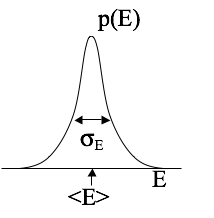
\includegraphics[width=\textwidth]{StatMech_figures/image094}
\caption{\label{fig:distn}Schematic of the distribution of energies in the canonical ensemble.}
\end{figure}

The standard deviation of the energy is the
root-mean-square difference of each configuational energy from the
average. It is easy to show that this can be expressed as the difference
in the ``average square energy'' and the ``square of the average
energy''
\begin{align*}
{\sigma _E} &= {\left\langle {{{\left( {E - \left\langle E \right\rangle } \right)}^2}} \right\rangle ^{1/2}}\\
 &= {\left[ {\left\langle {{E^2}} \right\rangle  - {{\left\langle E \right\rangle }^2}} \right]^{1/2}}
\end{align*}


We recently encountered the latter expression in our discussion of the
heat capacity \emph{C\textsubscript{V}}. Thus
\[{\sigma _E} = kT{({C_V}/k)^{1/2}}\]
The important measure is the standard deviation relative to the mean
\[\frac{{{\sigma _E}}}{{\left\langle E \right\rangle }} = \frac{{kT{{({C_V}/k)}^{1/2}}}}{{\left\langle E \right\rangle }} = \frac{{{\rm O}({N^{1/2}})}}{{{\rm O}(N)}} = {\rm O}({N^{ - 1/2}})\]
Here we apply the experimental observation that the heat capacity is an
extensive property. For a macroscopic system, the ratio is of order
10\textsuperscript{-11}: the likelihood of observing a microstate that
differs from the average by one standard deviation is about one in one
trillion. This indicates a very sharply peaked distribution of energies,
for which the mean is completely sufficient for its characterization.
For molecular simulation, the story is very different, and we see that
we can expect to see fluctuations in the energy of order 1 to 10\% when
sampling the relevant members of the ensemble. 
%Illustration 10 presents an applet that demonstrates the change in the magnitude of fluctuations with system size.

A related issue is the matter of equivalence of ensembles. The question
here could be phased thus:

\begin{itemize}
\item
  if I take a measurement of the pressure in a canonical ensemble at
  some volume;
\item
  and then input that pressure to an isothermal-isobaric ensemble;
\item
  will the NPT average of the volume equal the original
  canonical-ensemble volume?
\end{itemize}

The answer is yes, but only for a sufficiently large system. Averages
from different ensembles are consistent only to within quantities of
order 1/\emph{N}. We can demonstrate the discrepancy with a simple
example based on the ideal gas. The potential energy of an ideal gas is
defined to be zero: $U({{\bf{r}}^N}) \equiv 0$. Consequently, the canonical ensemble partition
function can be evaluated analytically:
\begin{align*}
{Q_{id}} &= \frac{1}{{{h^{dN}}N!}}\int {d{{\bf{p}}^N}\int {d{{\bf{r}}^N}} {e^{ - \beta K({{\bf{p}}^N})}}} \\
 &= \frac{{{V^N}}}{{{\Lambda ^{dN}}N!}}
\end{align*}
and the equation of state is easily derived:
\begin{align*}
{P_{\rm id}} &= kT\frac{{\partial \ln {Q_{\rm {id}}}}}{{\partial V}}\\
 &= \frac{{NkT}}{V}
\end{align*}
We could instead develop this result in the isothermal-isobaric
ensemble. The partition function there is
\begin{align*}
\Delta  &= \int\limits_0^\infty  {dV{e^{ - \beta PV}}\frac{1}{{{h^{dN}}N!}}\int {d{{\bf{p}}^N}\int {d{{\bf{r}}^N}} {e^{ - \beta E({{\bf{p}}^N},{{\bf{r}}^N})}}} } \\
 &= \int\limits_0^\infty  {dV{e^{ - \beta PV}}\frac{{{V^N}}}{{{\Lambda ^{dN}}N!}}} \\
 &= \frac{1}{{{{(\beta P)}^{N + 1}}{\Lambda ^{dN}}}}
\end{align*}
The corresponding equation of state is given by
\begin{align*}
V &=  - \frac{{\partial \ln \Delta }}{{\partial (\beta P)}}\\
 &= \frac{{N + 1}}{{\beta P}}
\end{align*}
from which
\[{P_{\rm ig}} = \frac{{NkT}}{V} + \frac{\rho }{N}\]
where $\rho = N/V$ is the number density. Clearly this expression differs
from the canonical-ensemble result, but by a factor that vanishes in the
thermodynamic limit of infinite $N$.

\end{document}
